\documentclass {article}
\usepackage{amsfonts}
\usepackage{amsmath}
\usepackage{amssymb}
\usepackage{algorithm}
\usepackage{tikz}
\usetikzlibrary{positioning, calc}
\usepackage{algpseudocode}
\usepackage[top=1in, bottom=1in, left=1in, right=1in]{geometry}


\begin{document}
\pagenumbering{gobble}
\begin{center}
\textbf{Euklidischer Algorithmus\\}
\textbf{Proseminar Informatik ``Algorithms Unplugged''}\\
am Institut f\"ur Theoretische Informatik\\
Leibniz Universit\"at Hannover\\
\end{center}
\begin{flushright}
\textit{Bharat Ahuja\\Wintersemester 2014/15}
\end{flushright}

\noindent\makebox[\linewidth]{\rule{\paperwidth}{0.4pt}}

\vspace*{10pt}
Der euklidische Algorithmus ist ein Algorithmus, mit dem sich der \underline{gr\"o{\ss}te gemeinsame Teiler} (\textit{g.g.T.}) zweier nat\"urlicher Zahlen berechnen l\"asst. Diesen Algorithmus hat Euklid ca. 300 \textit{v.Chr.} in \textit{Buch VII -- Die Elemente} (Proposition 1 und 2) als einen geometrischen Algorithmus vorgestellt.
\\

Die Berechnung vom \textit{g.g.T.} ist relevant f\"ur die Gruppierung von Objekten und das Pr\"ufen auf Teilerfremdheit von Zahlen.
 
Die Teilerfremdheit zweier Zahlen kann man alternativ durch das Vergleichen der Primfaktoren \"uberpr\"ufen.
	$$ggT(a,b) = \prod_{i \in \mathbb{N}} p_{i}^{min(a_i,b_i)}$$ wobei $p_{i} \in \mathbb{P}$.
Die Bestimmung der Primfaktorzerlegung einer Zahl liegt aber in NP.\\

Euklid hat damals den folgenden Algorithmus vorgestellt.\\

\textsc{LangsamEuklid}: Gegeben $a,b \in \mathbb{N}$
\begin{algorithmic}[1]
\While {$a\neq b$}
	\State Falls $a$ gr\"o{\ss}er ist als $b, a\gets a-b$
	\State Falls $b$ gr\"o{\ss}er ist als $a, b\gets b-a$
\EndWhile
	\State Gib den gemeinsamen Wert der Zahlen aus
\end{algorithmic}
\vspace{10pt}
\begin{center}
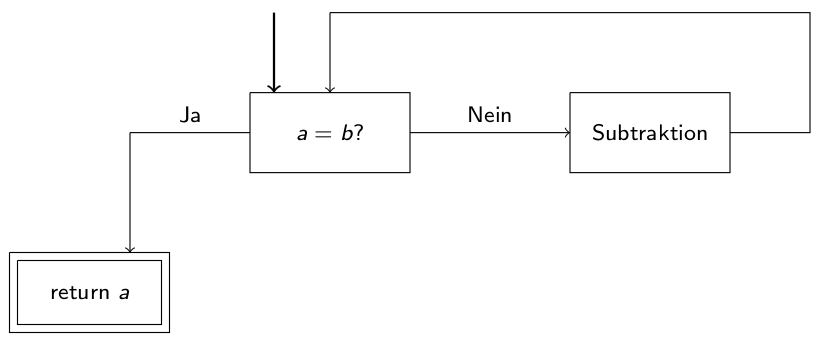
\includegraphics[scale=0.4]{langsamEuklid}
\end{center}
Dieser Algorithmus braucht viele \"uberfl\"ussige Schritte, die man weglassen m\"ochte, wenn eine der beiden Zahlen wesentlich gr\"o{\ss}er ist.

Den Algorithmus sollte man deswegen verbessern und so erhalten wir den modernen Euklidischen Algorithmus.
\newpage
	\textsc{Euklid}: Gegeben $a,b \in \mathbb{N}$
	 \begin{algorithmic}[1]
		\While {$b>0$}
		\State berechne $q,r$ mit $a=q\cdot b+r$, wobei $0\leq r < b$
		\State $a\gets b, b\gets r$
		\EndWhile
		\State \textbf{return} $a$
	\end{algorithmic}	
	\begin{center}
	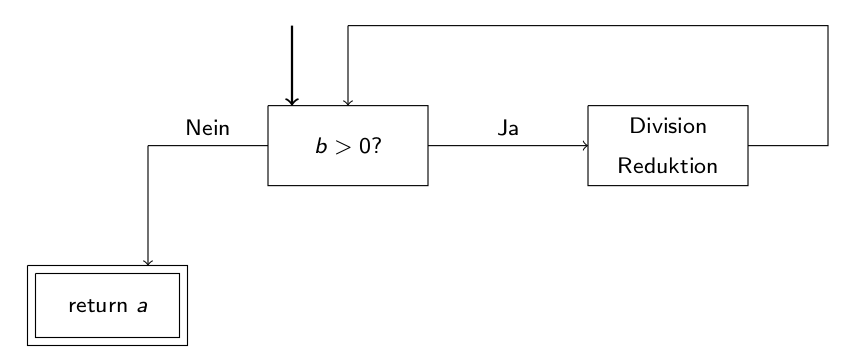
\includegraphics[scale=0.4]{euklid}
	\end{center}
	\vspace{10pt}
	$2\cdot \log_2{a}$ ist eine obere Schranke an der Anzahl an Iterationen von \textsc{Euklid}.
	
	Dieser Algorithmus ist nat\"urlich viel effizienter als \textsc{LangsamEuklid}, wo die obere Schranke an Iterationen $a+b$ lautet, weil man mehrfache Subtraktionen zusammengefasst hat.\\


Betrachtet man den Worst-Case f\"ur diesen Algorithmus, dann stellt man fest, je schneller die Reste fallen, desto fr\"uher terminiert der Algorithmus. D.h. die Fibonacci-Zahlen bilden den ung\"unstigsten Fall f\"ur diesen Algorithmus, weil alle Quotienten den kleinstm\"oglichen Wert annehmen, und dadurch die Reste sehr langsam fallen.

Im Kern ist der Euklidische Algorithmus effizient, weil nach jeder Iteration immer nur der Divisionsrest relevant ist.\\
Zur Veranschaulichung : Pr\"uft man die Zahlen $938631347$ und $2$ auf Teilerfremdheit, so achtet man intuitiv auch nur auf den Divisionsrest.
	$$\Rightarrow T_{b} = \frac{1}{b} \sum_{0 < k\leq b} T(k,b)$$ wobei $T_{b}$ die durchschnittliche Anzahl an Divisionen ist, wenn man eine zuf\"allige Zahl auf Teilerfremdheit mit $b$ pr\"ufen m\"ochte.

Ausserdem gilt,
	$$T_n \approx H_n$$
	\begin{flushright}
	wobei $H_n$ die $n$-te harmonische Zahl ist.	
	\end{flushright}	
\vspace*{10pt}
Literaturverzeichnis :
\begin{itemize}
\item \textit{The Art of Computer Programming: Band 1} Kapitel 1.1
\item \textit{The Art of Computer Programming: Band 2} Kapitel 4.5.2
\end{itemize}
\end{document}
